\documentclass[journal]{IEEEtran}
%
% If IEEEtran.cls has not been installed into the LaTeX system files,
% manually specify the path to it like:
% \documentclass[journal]{../sty/IEEEtran}

\makeatletter
\def\markboth#1#2{\def\leftmark{\@IEEEcompsoconly{\sffamily}\MakeUppercase{\protect#1}}%
\def\rightmark{\@IEEEcompsoconly{\sffamily}\MakeUppercase{\protect#2}}}
\makeatother

\usepackage[latin1]{inputenc}
\usepackage[T1]{fontenc}
\usepackage{cite}
\usepackage{graphicx}
\usepackage{url}
\usepackage[norsk,english]{babel}
\usepackage{amsmath}
\usepackage{verbatim}
\usepackage{varioref}
\usepackage{color}
\usepackage{listings}

%\usepackage[cmex10]{amsmath}
%\usepackage{algorithmic}
%\usepackage{array}
%\usepackage{mdwmath}
%\usepackage{mdwtab}
%\usepackage[tight,footnotesize]{subfigure}
%\usepackage[caption=false]{caption}
%\usepackage[font=footnotesize]{subfig}
%\usepackage[caption=false,font=footnotesize]{subfig}
%\usepackage{fixltx2e}
%\usepackage{stfloats}

% correct bad hyphenation here
\hyphenation{net-works}


\begin{document}

\title{Implementation of CacheCast\\ in the ns-3 network simulator}

\author{Kanat~Sarsekeyev,~
        Bekzahan~Kassymbekov,~
        Rizwan~Ali~Ahmed,~
        and~Dag~Henning~Liodden~S�rb�}% <-this % stops a space

% \thanks{J. Doe and J. Doe are with Anonymous University.}% <-this % stops a space
% \thanks{Manuscript received April 19, 2005; revised January 11, 2007.}}

% The paper headers
% \markboth{Journal of \LaTeX\ Class Files,~Vol.~6, No.~1, January~2007}%
% {Shell \MakeLowercase{\textit{et al.}}: Bare Demo of IEEEtran.cls for Journals}


%%---------------------------------------------------------------------------%%
% make the title area
\maketitle


\begin{abstract}
Na na na na na na na na na na... B���TM����n!!!!
\end{abstract}


% \begin{IEEEkeywords}
% IEEEtran, journal, \LaTeX, paper, template.
% \end{IEEEkeywords}


\section{Introduction}
\IEEEPARstart{T}{he} goal of this project... Bla bla... 



\section{CacheCast}


\section{ns-3}
The ns-3 simulator is a discrete-event network simulator. It is an open-source project written in C++. ns-2 is a version prior to ns-3, which is a new simulator that does not support the ns-2 APIs. Some models from ns-2 have already been ported from ns-2 to ns-3, and some has not yet been implemented in ns-3.

\subsection*{Abstractions}
Before we start explaining the implementation of CacheCast in ns-3, it is important to understand abstractions and terms that are used in ns-3

\subsubsection{Node}
In ns-3 devices like host and end-user are represented as abstractions of nodes by the class \texttt{Node}. This class provides management of how these devices will be represented in simulations. 

\subsubsection{Application}
Application is abstractions of user programs that are suppose to produce activity on nodes to be simulated. This is represented by the class \texttt{Application}, which provides methods for managing the representations of applications in simulations.

\subsubsection{Channel}
In ns-3, each Node are connected by a connection that are represented by a communication channel. This abstraction is represented by class \texttt{Channel}, which provides methods for managing communication subnetwork objects and connecting nodes to them.

\subsubsection{NetDevice}
Net device abstraction covers both the software driver and the simulated hardware. A net device is  more or less "installed" in a Node in order to enable the Node to communicate with other Nodes in the simulation via Channels. Node may be connected to more than one Channel via multiple NetDevices. This abstraction is represented by class \texttt{NetDevice} which provides management of connections to Node and Channel.

\subsubsection{Topylogy Helpers}
In a simulated network, connections between Nodes, NetDevices and Channels needs to be arranged. NetDevices needs to be attached on Nodes, Node protocol-stack needs to be configured and a communication channels need to be defined between NetDevices and so on. Topology helpers are used to arrange these attachments as easy as possible on a large scale.

\section{Application programming interface (API)\label{api}} % HOW TO USE IT
We have now talked about the general design of CacheCast and about the details 
of the ns-3 network simulator. In this section we will explain how the CacheCast 
system is used by script authors. bla bla ...


\subsection{Services provided to applications}
Since end-to-end cachecast connections are handled by different sockets, the send procedure requires a sequence of send-requests (corresponding to each socket) to transmit packets to all client. A multiple-send-request from application layer requires a container of sockets, so the application can send duplicated packets through / to all sockets in the container. 

Since a such socket container is not supported by transport layer and nor a part of a application-layer, we chose to implement a CacheCast Application Programming Interface in the class \texttt{CacheCast}. This interface will not only support the socket container, but also systemcall \texttt{Msend()} would be provided to the application. This is much more practical than having a static systemcall called by the application.

\begin{footnotesize}
\begin{lstlisting}[language=C]
--------------------------------------------------
std::vector <Ptr <Socket> > m_sockets; 
std::vector <Ptr <Socket> > m_failed;
--------------------------------------------------
\end{lstlisting}
\end{footnotesize}

The socketcontainer itself is implemented as a vector of sockets (\texttt{m\_sockets}), which contains sockets added by application. In addition to vector \texttt{m\_sockets} we chose to have another vector \texttt{m\_failed} to provide the application the knowledge of sockets that failed during the msend procedure.

\begin{footnotesize}
\begin{lstlisting}[language=C]
--------------------------------------------------
void AddSocket(Ptr<Socket> socket);
void RemoveSocket(Ptr<Socket> socket);
    
void Merge(CacheCast cc);
   
Iterator Begin (void) const;
Iterator End (void) const;
 
Iterator BeginFailedSockets (void) const;
Iterator EndFailedSockets (void) const;

bool Msend(Ptr<Packet> packet);
--------------------------------------------------
\end{lstlisting}
\end{footnotesize}
In order to maintain the container of sockets, some facilities are provided to the application. It is necessary for the application to add or remove sockets in the container. And the possibility to merge two or more socketcontainers might also become handy.

\begin{footnotesize}
\begin{lstlisting}[language=C]
--------------------------------------------------
std::vector<Address>::const_iterator it;

CacheCast cc;

for (it = m_address.begin();
it < m_address.end(); ++it)
{
  Ptr<Socket> socket = Socket::CreateSocket 
  (GetNode (), TypeId::LookupByName 
  ("ns3::UdpSocketFactory"));
  socket->Bind();
  socket->Connect (*it);
  cc.AddSocket (socket);
}
for (it = m_address.begin();
 it < m_address.end(); ++it) 
{
  Ptr<Socket> socket = Socket::CreateSocket 
  (GetNode (), TypeId::LookupByName 
  ("ns3::UdpSocketFactory"));
  socket->Bind();
  socket->Connect (*it);
  cc2.AddSocket (socket);
}

cc.Merge(cc2);

Ptr<Packet> packet = Create<Packet> (1472);

if(!cc.Msend(packet)){
  CacheCast::Iterator vItr = cc.BeginFailedSockets();
  while ( vItr != cc.EndFailedSockets() )
  {
    cc.RemoveSocket( (*vItr) );
    vItr++;
  }    
}
--------------------------------------------------
\end{lstlisting}
\end{footnotesize}

\subsection{Helpers}



\section{Implementation details} % HOW IT WORKS
In the previous section we looked at the implementation of CacheCast in ns-3 
from the user perspective. In this section we will dig deeper into the 
implementation details and look at the implementation from a developer 
perspective. First we will take a birds view of the design of implementation to 
get a general overview of how it works. Then we look at common data structures 
used throughout the implementation. At last we elaborate on the specific 
implementation details of each part.

\subsection{General overview}
The implementation of CacheCast in ns-3 (as in the general design of CacheCast) 
consists of three main parts; server support, CMU and CSU. As explained in the 
previous section, to support CacheCast, packets are sent with the 
CacheCast::Msend() function in the ns-3 applications on the server node. Then 
the packets traverse the network layers and is intercepted by the CacheCastNetDevice. In 
this CacheCastNetDevice a CacheCastServerUnit is installed which adds a 
CacheCastHeader to the packets and truncates packets with redundant payload. The 
packets then traverse the channel and is received by a new CacheCastNetDevice 
on the other end. In this CacheCastNetDevice a CacheStoreUnit is 
installed which adds payload to the truncated packets and remove the 
CacheCastHeader. The packets are then handled as normal IP packets in the node. 
If the packet is destined for another node, it is again intercepted by a new 
CacheCastNetDevice in which a CacheManagementUnit is installed. This unit adds 
the CacheCastHeader to the packet and truncates packets with redundant payload. 
The packets then traverse a new channel and is received by a new 
CacheCastNetDevice with a CacheStoreUnit installed. This process is continued 
for each node supporting CacheCast on the packet's path to its destination. An 
graphical overview of this structure can be seen in figure \ref{fig_overview}.

\begin{figure}[!t]
\centering
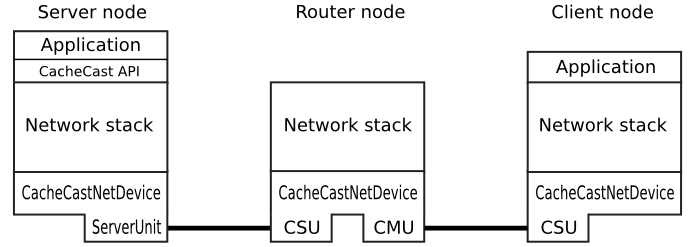
\includegraphics[width=3.5in]{overview}
\caption{The structure of the CacheCast system in ns-3}
\label{fig_overview}
\end{figure}


\subsection{Common data structures and classes}
In this section we explain the common data structures used by the different 
parts of the ns-3 implementation of CacheCast.

\subsubsection{CacheCast header}
The CacheCast header is represented in ns-3 as a class named CacheCastHeader. 
This class is derived from the general ns3::Header class. The class contains the 
same members as the header described in the design of CacheCast, namely payload 
ID, payload size and index. An overview of the %CacheCast related elements of the 
CacheCastHeader is given in the listing below.

\begin{footnotesize}
% -------------- WIDTH ----------------------------]
\begin{lstlisting}[language=C, frame=single]
#include "ns3/header.h"

namespace ns3 {
class CacheCastHeader : public Header
{
public:
  CacheCastHeader ();
  CacheCastHeader (uint32_t payloadId, 
    uint16_t payloadSize, uint32_t index);
  uint32_t GetPayloadId (void) const;
  uint16_t GetPayloadSize (void) const;
  uint32_t GetIndex (void) const;
  void SetPayloadId (uint32_t payloadId);
  void SetPayloadSize (uint16_t payloadSize);
  void SetIndex (uint32_t index);

  static TypeId GetTypeId (void);
  TypeId GetInstanceTypeId (void) const;
  void Print (std::ostream &os) const;
  uint32_t GetSerializedSize (void) const;
  void Serialize (Buffer::Iterator start) const;
  uint32_t Deserialize (Buffer::Iterator start);
private:
  uint32_t m_payloadId;
  uint16_t m_payloadSize;
  uint32_t m_index;
};
}
\end{lstlisting}
\end{footnotesize}


\subsubsection{CacheCast packet tag}
In ns-3 one have the possibility to add packet tags to packets in order to store 
information on a packet level. In the implementation of CacheCast we use packet 
tags to store CacheCast related values when the packet is processed in a node 
(where the CacheCast header is not present). These values are the payload ID and 
the payload size. These are necessary for the CMU in order to uniquely identify 
CacheCast packets and handle them correctly. 

% The CacheCastTag is added by the 
% Msend() function on the server and the CSU on the other nodes. It is removed by 
% the CacheCastServerUnit and the CMU TODO DO WE NEED TO REMOVE THE TAG?

\subsubsection{CacheCastUnit}
The CacheCastUnit class is an abstract base class which should be derived from 
in order to support different packet handling schemes in CacheCast. This class 
contains only one CacheCast related function named \textsf{virtual bool 
HandlePacket (Ptr<Packet> p)}. This function takes a pointer to a packet which 
it can modify. The derived classes is supposed to override this function. There 
are currently three derived classes from the CacheCastUnit base class; 
CacheCastServerUnit, CacheManagementUnit and CacheStoreUnit. These classed will 
be explained later in this document.

\subsubsection{CacheCastNetDevice}
In the ns-3 network simulator the abstraction of the physical and the data link 
layer is modeled by a NetDevice. This NetDevice receives a packet from the 
network layer, adds link layer headers, and puts the packet onto the channel. 
Because of this design we have chosen to create a new NetDevice which supports 
CacheCast. This NetDevice is called CacheCastNetDevice and is strongly based on 
the PointToPointNetDevice. In the first attempt of creating this NetDevice we 
tried to make CacheCastNetDevice a derived class of the PointToPointNetDevice. 
This proved difficult due to the design of the PointToPointNetDevice. There was 
no way to get to the packet after the transmission queue and before it was 
transmitted onto the link, which is crucial for the CacheCast technique. Because 
of this we chose to copy much of the code from PointToPointNetDevice and adapt 
it to the CacheCast scenario. Since CacheCast is only supported on 
point-to-point links the CacheCastNetDevice need not be generalized into 
arbitrary link level technologies.

The CacheCastNetDevice is used both on the server and on nodes and it is used 
together with the ServerUnit, the CMU and the CSU. To support these different 
scenarios we have added a senderUnit and a receiverUnit object to the class. 
These objects are derived from the CacheStoreUnit class so their purpose is to 
modify packets. The main idea of CacheCast is to intercept the packets before 
they are transmitted onto the link to remove redundant payload. In our 
implementation this interception is done in the 
CacheCastNetDevice::TransmitStart() function. The packets need to be intercepted 
also on the receiver side, and this is done in CacheCastNetDevice::Receive(). In 
these functions the HandlePacket() function of the senderUnit and receiverUnit 
is called, respectively. So this is where the actual CacheCast packet 
modification happens. More will be said in the following sections about how this 
packet modification is done.

In order to have a channel to connect to the new CacheCastNetDevice we had to 
create an adapted version of the PointToPointChannel named CacheCastChannel. The 
only reason for this class is to support the CacheCastNetDevice. No CacheCast 
related packet handling is done in this class.

Now we have looked into the common data structures used in our 
implementation. Let us in the following sections go more into detail of the 
actual packet handling mechanisms of the CacheCast system. First we take a look 
into the server part and then we continue with the networking part of the 
implementation.


\subsection{Server support}
The CacheCast system relies on support from the server in order to remove 
redundant payload in the network. This server support should send all packets 
sequentially onto the link and truncate all packets beside the first one. This 
removes redundant payload from the link and forms a packet train.

The general design of the CacheCast server support consists mainly of two parts; 
the programming interface to the applications and the underlying packet handling 
mechanism. The implementation in ns-3 closely resembles this division. The 
implementation details of the API exposed to the applications is discussed in 
the next section while the underlying handling of packets is discussed in 
section \ref{serverunit}.


\subsubsection{Details of the API implementation}


TODO write about CacheCastPid

\begin{footnotesize}
% -------------- WIDTH ----------------------------]
\begin{lstlisting}[language=C, frame=single]
bool 
CacheCast::Msend (Ptr<Packet> packet)
{

  bool successful = true;
  std::vector<Ptr <Socket> >::iterator socket;

  if (m_sockets.size() == 0)
    return true;

  Ptr<CacheCastPid> pid = m_sockets[0]->GetNode ()->GetObject<CacheCastPid> ();
  
  NS_ASSERT_MSG (pid, 
  "A CacheCast server must have a CacheCastPid object");
  
  uint32_t payloadId = pid->CalculateNewPayloadId ();

  for(socket = m_sockets.begin(); 
  socket != m_sockets.end(); ++socket)
  {        
    // if DCCP gets supported handle it also
    NS_ASSERT_MSG ((*socket)->GetSocketType () == Socket::NS3_SOCK_DGRAM,
    "CacheCast supports only UDP sockets");
    
    Ptr<Packet> p = packet->Copy (); 

    CacheCastTag tag (payloadId, p->GetSize ());
    p->AddPacketTag (tag);        

    if((*socket)->Send(p) < 0)
    {
      successful = false;
      SetFailedSocket (socket_index);
    }
  }

  return successful; 
}

\end{lstlisting}
\end{footnotesize}

\subsubsection{Underlying packet handling mechanism\label{serverunit}}
The tasks of the underlying packet handling mechanism on a CacheCast supported 
server is to ensure that the packets are put onto the link in a tight chain and 
to add the CacheCast header to each packet. In the Linux implementation of 
CacheCast this mechanism is handled by a kernel module located between the 
network layer and the link layer. As previously explained we have chosen to 
create a new CacheCastNetDevice in which we can install different packet 
handling mechanisms. This is where the CacheCast packet modification will 
happen.

On the server an object of a class CacheCastServerUnit is added as a senderUnit 
to each CacheCastNetDevice. The CacheCastServerUnit::HandlePacket() function 
does the actual packet modification and its contents is listed below.

\begin{footnotesize}
% -------------- WIDTH ----------------------------]
\begin{lstlisting}[language=C, frame=single, showstringspaces=false]
bool
CacheCastServerUnit::HandlePacket (Ptr<Packet> p)
{
  NS_LOG_FUNCTION (p);

  CacheCastTag tag;
  bool hasTag = p->RemovePacketTag (tag);
  NS_ASSERT_MSG (hasTag, "No CacheCast packet tag");

  CacheCastHeader cch (tag.GetPayloadId (),
    tag.GetPayloadSize (), 0);

  /* Invalidate the current payload ID
     after one second */
  if (Simulator::Now ().GetSeconds () - m_timeStamp
    > 1.0)
  {
    NS_LOG_DEBUG ("CacheCast server table 
        invalidated");
    m_invalid = true;
    m_timeStamp = Simulator::Now ().GetSeconds ();
  }

  if (m_payloadId == tag.GetPayloadId ()
      && !m_invalid)
  {
    // remove payload
    p->RemoveAtEnd (tag.GetPayloadSize ());
    cch.SetPayloadSize (0);
  }
  else
  {
    // new payload ID
    m_payloadId = tag.GetPayloadId ();
    m_invalid = false;
  }

  p->AddHeader (cch);

  return true;
}
\end{lstlisting}
\end{footnotesize}

The code itself should be rather self-explanatory. First we check if the payload 
has been in the table for 1 second, and if it has we invalidate this payload ID from the 
table. The reason for doing this is to support wrapping of payload IDs. The 
design of CacheCast specifies that a specific payload ID should be invalidated 
if it has been present in a table for 1 second or more. The rest of the code 
modifies the packet. If the packet's payload ID is not present in the table it 
is added and no further changes are done to the packet payload. If a payload ID 
is present in the table the payload is removed from the packet and the payload 
size field in the CacheCastHeader is set to 0. At last the CacheCastHeader is 
added to the packet. The HandlePacket() function returns control back to the 
CacheCastNetDevice::TransmitStart() function which continues to transmit the 
packet onto the link.

The design of CacheCast demands that the packets forming a packet train is put 
in tight sequential order on the link. In order to obtain a continuous packet 
train all packets with the same payload should be transmitted in one batch onto 
the link. In the implementation of CacheCast in Linux this is handled by a 
separate packet queue in the CacheCast kernel module to overcome the issue of 
the multiprocess nature of modern operating system. In ns-3 all code is executed 
in sequential order with no interruption. Also computing time on the nodes is 
not modeled in ns-3. Thus in our implementation we do not need to batch the 
packets at link layer level. The batching of sockets done in the application domain is 
sufficient enough to form continuous packet trains.



only one entry in table

index to 0





\subsection{Network support}



\section{Evaluation}


\section{Conclusion}
The conclusion goes here.



% \appendices
% \section{Proof of the First Zonklar Equation}
% Appendix one text goes here.
% 
% % you can choose not to have a title for an appendix
% % if you want by leaving the argument blank
% \section{}
% Appendix two text goes here.


\section*{Acknowledgment}
The authors would like to thank their always positive and helpful supervisor Piotr 
Srebrny for useful guidelines and input in time of need.

%\bibliographystyle{IEEEtran}
% argument is your BibTeX string definitions and bibliography database(s)
%\bibliography{IEEEabrv,../bib/paper}

\section*{Contributions}

\begin{tabular}{|l||p{3.4cm}|}
\hline
Kanat~Sarsekeyev & ...\\
\hline
Bekzahan~Kassymbekov & ...\\
\hline
Rizwan~Ali~Ahmed & ...\\
\hline
Dag~Henning~Liodden~S�rb� & bla bla\\
& bla\\
\hline
\end{tabular}


%%---------------------------------------------------------------------------%%
\end{document}


% EXAMPLES

%\begin{figure}[!t]
%\centering
%\includegraphics[width=2.5in]{myfigure}
%\caption{Simulation Results}
%\label{fig_sim}
%\end{figure}

%\begin{table}[!t]
%% increase table row spacing, adjust to taste
%\renewcommand{\arraystretch}{1.3}
% if using array.sty, it might be a good idea to tweak the value of
% \extrarowheight as needed to properly center the text within the cells
%\caption{An Example of a Table}
%\label{table_example}
%\centering
%% Some packages, such as MDW tools, offer better commands for making tables
%% than the plain LaTeX2e tabular which is used here.
%\begin{tabular}{|c||c|}
%\hline
%One & Two\\
%\hline
%Three & Four\\
%\hline
%\end{tabular}
%\end{table}

